\section{Model with noise and discretization}

There are several sources of noise in a micro-bolometer setup:
\begin{itemize}
\item Thermal noise in the resistances,
\item Flicker noise in resistances,
\item Burst noise,
\item Thermal fluctuations in the bolometer temperature,
\item Noise in incident IR radiation,
\item Noise in read out circuits.
\end{itemize}

In this report we shall only consider the first two types of noises,
thermal and flicker noise in resistances.

\subsection{Thermal noise}

Any resistance with a temperature $T$ above zero, will cause the
charge carriers in the material to fluctuate. The fluctuations are
independent of each other, and will generate a current with a
voltage. This phenomenon is referred to as thermal noise, but is also
known as white noise and Johnson noise. This type of noise was first
discovered by the Swedish engineer John
B. Johnson~\cite{PhysRev.32.97}, and his colleague Harry Nyquist, also
swedish, provided a theory for the noise based on statistical
physics\cite{PhysRev.32.110}. One of the characteristics of the noise,
is the flat power spectrum for all most all frequencies, which is also
characteristic for white light.

In electrical circuits, thermal noise is commonly modeled as an additional
power source in series with the resistance, see Figure~\ref{fig:johnsonEquivalentNoise}.
\begin{figure}
  \centering
  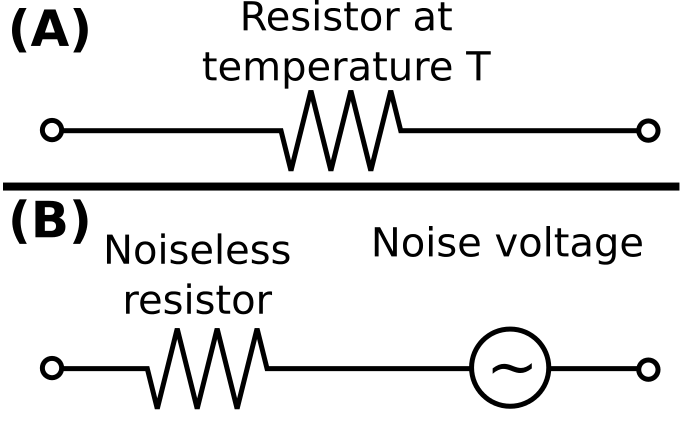
\includegraphics[width=0.5\textwidth]{gfx/JohnsonNoiseEquivalentCircuits.png}
  \caption{Equivalent model for thermal noise in a resistor.}
  \label{fig:johnsonEquivalentNoise}
\end{figure}
Due to the random nature of the additional power source, it is not
possible to predict the instataneous voltage produced, but instead the
average behavior. Nyquist\cite{PhysRev.32.110} found that the power
spectrum of thermal noise to be
\begin{equation}
  \label{eq:power_spectrum_white_noise}
  S(f) = 4 k_B T R,
\end{equation}
where $k_B$ is the Boltzmann constant, $T$ is the temperature of the
resistance, and $R$ is the resistance. The total contribution of the
noise source is then calculated by summing up the contribution from
each frequency component.
\begin{equation}
  \label{eq:2}
  \E \left[ V^2 \right] = \int_B S(f) \mathrm(d) f,
\end{equation}
where $B$ is the bandwidth of the circuit.

% The mean square square voltage o

A statistical model commonly used to white noise is a stationary stochastic
process where the auto-correlation function is
\begin{equation}
  \label{eq:autocorrelation_white_noise}
  R(s,t)={\frac {\operatorname {E} [(X_{t}-\mu _{t})(X_{s}-\mu
      _{s})]}{\sigma _{t}\sigma _{s}}} =
  \begin{cases}
    \sigma_{t}^2 , \quad t = s, \\
    0 , \quad t \neq s
  \end{cases}
\end{equation}
meaning that the process is uncorrelated in time. A distribution that
can be used for this process is the Gaussian distribution
$\mathcal{N}(0, \sigma)$.

\subsection{Flicker Noise}

Another type of noise source that exists in circuits is the flicker
noise, or also known as low frequency noise, 1/$f$ noise or pink noise. The power
spectrum of the Flicker noise is
\begin{equation}
  \label{eq:power_spectrum_flicker_noise}
  S(f) \propto \frac{k}{f^{\alpha}}.
\end{equation}
where $\alpha \in [0.5, 1.5]$ and $k$ is a material constant.

One explanation of the occurrence of the flicker noise in resistors is
that the charge carriers get trapped in capture sites of the
conductor, and are then released with variable rates. This was first
explained by Schottky for flicker noise in vacuum tubes~\cite{PhysRev.28.74}.
% The noise occurs in all types of electrical devices and can be caused by
% impurities in the conductors and fluctuating configurations of defects
% in metals.


\subsection{Model with noise}

To compensate for the noise in the read-out circuit, one first has to
determine how noise enters the differential equation governing the
behavior of the system. The assumption we make is that the noise is
additive in the bolometer resistance. By using the model in
Figure~\ref{fig:johnsonEquivalentNoise}, we redefine the voltage over
the bolometer resistance as
\begin{equation}
  \label{eq:randomvariable_transformation}
  V \rightarrow V_0 + \Delta V,
\end{equation}
where $V_0$ is the noise-less resistance over the voltage, and $\Delta
V$ is the random variable representing the random fluctuations in the
voltage. If there are several noise sources present in the resistance
that are uncorrelated and additive, the resulting voltage is then
\begin{equation}
  \label{eq:randomvariable_transformation}
  V \rightarrow V_0 + \sum_i \Delta V_i.
\end{equation}
Thus, assuming that the Flicker noise and the thermal noise are
uncorrelated, they enter the voltage as two separate sources.


The heat equation in Equation~\eqref{eq:heat_balance_equation}, can
thus be modified to include the two noise sources as
\begin{equation}
  \label{eq:heat_balance_equation_noise}
  C\frac{dT}{dt}=\frac{(V_b(t) + \Delta V)^2}{R(T)}+ f(T),
\end{equation}
where $\Delta V$ is the added noise term, accounting for the
fluctuations in the resistance $R(T)$ and $f(T)$ are the other terms
in Equation~\eqref{eq:heat_balance_equation}. We assume that $\Delta V
\sim \mathcal{N} (0, \sigma)$.

\subsection{Discretization of the stochastic model}


The modified heat equation in~\eqref{eq:heat_balance_equation_noise}
needs to be discretized in the time domain to be numerically
simulated. We can rewrite~\eqref{eq:heat_balance_equation_noise} as
a stochastic differential equation
\begin{equation}
  \label{eq:heat_balance_equation_noise_SDE}
  CdT=\frac{1}{R(T)} (V_b^2(t) + 2 V_b(t) \Delta V + (\Delta V)^2)dt + f(T) dt,
\end{equation}
In the discretization scheme, the term $V_b(t) \Delta V dt $ is
written as $V_b(t) \Delta V \sqrt{\Delta t}$, where $\Delta t$ is the
step-length in the Euler scheme. This is done to keep the variance of
$\Delta V$ invariant of $\Delta t$. However, the term $(\Delta V)^2dt$
cannot be discretized in the same manner, and a simple approximation
is to set $(\Delta V)^2 dt \approx  \sigma^2$. Thus, discretized noisy
heat equation can be written as
\begin{equation}
  \label{eq:heat_balance_equation_noise_SDE_disc}
  C \Delta T=\frac{1}{R(T)} (V_b^2(t) \Delta t  + 2 V_b(t) \Delta V \sqrt{\Delta t}+ \sigma^{2}) + f(T) \Delta t
\end{equation}


%%% Local Variables:
%%% mode: latex
%%% TeX-master: "main"
%%% TeX-PDF-mode: 1
%%% TeX-PDF-via-dvips-ps2pdf: 1
%%% End:
